%%%%%%%%%%%%%%%%%%%%%%%%%%%%%%%%%%%%

\section{Considering categorical data}

%%%%%%%%%%%%%%%%%%%%%%%%%%%%%%%%%%%%

\subsection{Contingency tables and bar plots}

%%%%%%%%%%%%%%%%%%%%%%%%%%%%%%%%%%%%

\begin{frame}
\frametitle{Contingency tables}

A table that summarizes data for two categorical variables is called a \hl{contingency table}.

$\:$ \\
\pause
The contingency table below shows the distribution of survival and ages of passengers on the Titanic.

\begin{center}
\begin{tabular}{l l cc r}
					               & 			 & \multicolumn{2}{c}{{Survival}} \\
  \cline{3-4}
					               &			 & Died	 & Survived	& Total \\ 
  \cline{2-5}
\multirow{2}{*}{{Age}}& Adult & 1438  & 654 	  	& 2092 \\ 
  					             & Child & 52 	 & 57	 	    & 109\\ 
  \cline{2-5}
  					             & Total & 1490  & 711	    &  2201 \\
  \cline{2-5}
\end{tabular}
\end{center}
\end{frame}

%%%%%%%%%%%%%%%%%%%%%%%%%%%%%%%%%%%%

\begin{frame}
\frametitle{Bar plots}

A \hl{bar plot} is a common way to display a single categorical variable. A bar plot where proportions instead of frequencies are shown is called a \hl{relative frequency bar plot}.

\begin{center}
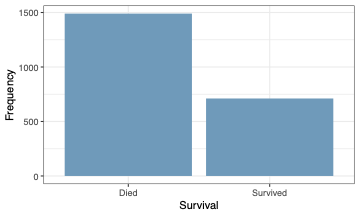
\includegraphics[width=0.45\textwidth]{2-2_categorical_data/figures/titanic_age_survival/titanic_bar}
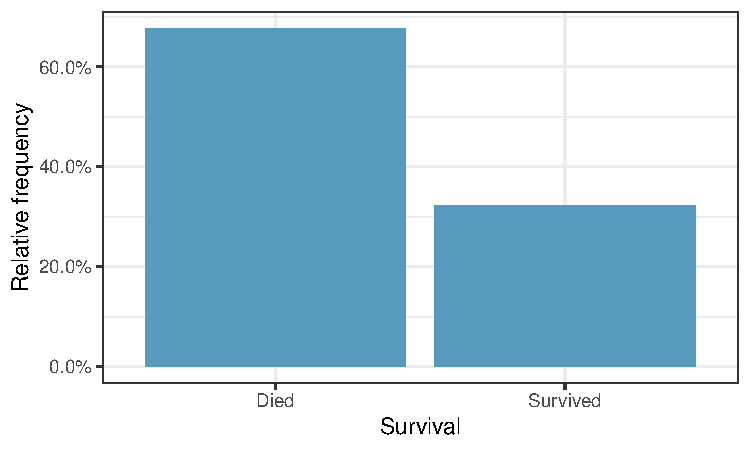
\includegraphics[width=0.45\textwidth]{2-2_categorical_data/figures/titanic_age_survival/titanic_rel_bar}
\end{center}

\pause

\dq{How are bar plots different than histograms?}

\soln{\pause{{\tiny Bar plots are used for displaying distributions of categorical variables,  histograms are used for numerical variables. The x-axis in a histogram is a number line,  hence the order of the bars cannot be changed. In a bar plot, the categories can be listed in any order (though some orderings make more sense than others, especially for ordinal variables.)}}}

\end{frame}

%%%%%%%%%%%%%%%%%%%%%%%%%%%%%%%%%%%%

\subsection{Row and column proportions}

%%%%%%%%%%%%%%%%%%%%%%%%%%%%%%%%%%%%

\begin{frame}
\frametitle{Choosing the appropriate proportion}

\dq{Does there appear to be a relationship between age and survival for passengers on the Titanic?}

\begin{center}
\begin{tabular}{l l cc r}
					               & 			 & \multicolumn{2}{c}{{Survival}} \\
  \cline{3-4}
					               &			 & Died	 & Survived	& Total \\ 
  \cline{2-5}
\multirow{2}{*}{{Age}}& Adult & 1438  & 654 	  	& 2092 \\ 
  					             & Child & 52 	 & 57	 	    & 109\\ 
  \cline{2-5}
  					             & Total & 1490  & 711	    &  2201 \\
  \cline{2-5}
\end{tabular}
\end{center}

\pause

To answer this question we examine the row proportions: 

\pause

\begin{itemize}

\item \% Adults who survived: 654 / 2092 $\approx 0.31$ \\

\pause

\item \% Children who survived: 57 / 109 $\approx 0.52$ \\

\end{itemize}

\end{frame}

%%%%%%%%%%%%%%%%%%%%%%%%%%%%%%%%%%%%

\subsection{Using a bar plot with two variables}

%%%%%%%%%%%%%%%%%%%%%%%%%%%%%%%%%%%%

\begin{frame}
\frametitle{Bar plots with two variables}

\begin{itemize}

\item \hl{Stacked bar plot:} Graphical display of contingency table information,
for counts.

\item \hl{Side-by-side bar plot:} Displays the same information by placing bars 
next to, instead of on top of, each other.

\item \hl{Standardized stacked bar plot}: Graphical display of contingency table 
information, for proportions.

\end{itemize}

\end{frame}

%%%%%%%%%%%%%%%%%%%%%%%%%%%%%%%%%%%%

\begin{frame}

\dq{What are the differences between the three visualizations shown below?}

\begin{center}
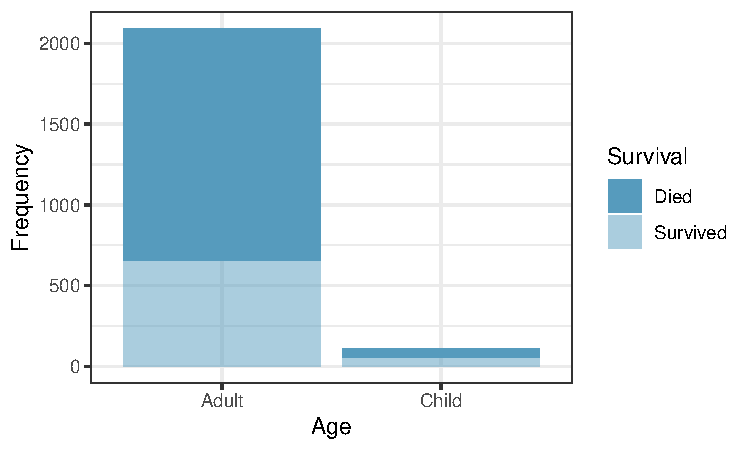
\includegraphics[width=0.5\textwidth]{2-2_categorical_data/figures/titanic_age_survival/titanic_seg_bar}
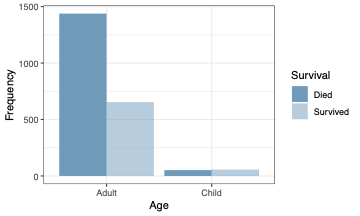
\includegraphics[width=0.5\textwidth]{2-2_categorical_data/figures/titanic_age_survival/titanic_seg_bar_dodge} \\
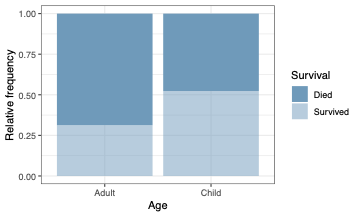
\includegraphics[width=0.5\textwidth]{2-2_categorical_data/figures/titanic_age_survival/titanic_rel_seg_bar}
\end{center}

\end{frame}

%%%%%%%%%%%%%%%%%%%%%%%%%%%%%%%%%%%%

\subsection{Mosaic plots}

%%%%%%%%%%%%%%%%%%%%%%%%%%%%%%%%%%%%

\begin{frame}
\frametitle{Mosaic plots}

\dq{What is the difference between the two visualizations shown below?}

\begin{center}
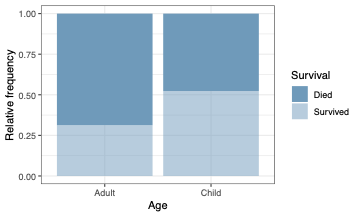
\includegraphics[width=0.5\textwidth]{2-2_categorical_data/figures/titanic_age_survival/titanic_rel_seg_bar}
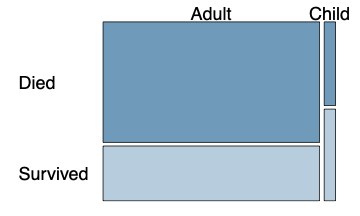
\includegraphics[width=0.5\textwidth]{2-2_categorical_data/figures/titanic_age_survival/titanic_mosaic}
\end{center}

\end{frame}

%%%%%%%%%%%%%%%%%%%%%%%%%%%%%%%%%%%%

\subsection{Pie charts}

%%%%%%%%%%%%%%%%%%%%%%%%%%%%%%%%%%%%

\begin{frame}
\frametitle{Pie charts}

\dq{Can you tell which order encompasses the lowest percentage of mammal species?}

\vspace{-0.5cm}

\begin{center}
\includegraphics[width=0.4\textwidth]{2-2_categorical_data/figures/mammal_pie_chart/mammal_pie_chart}
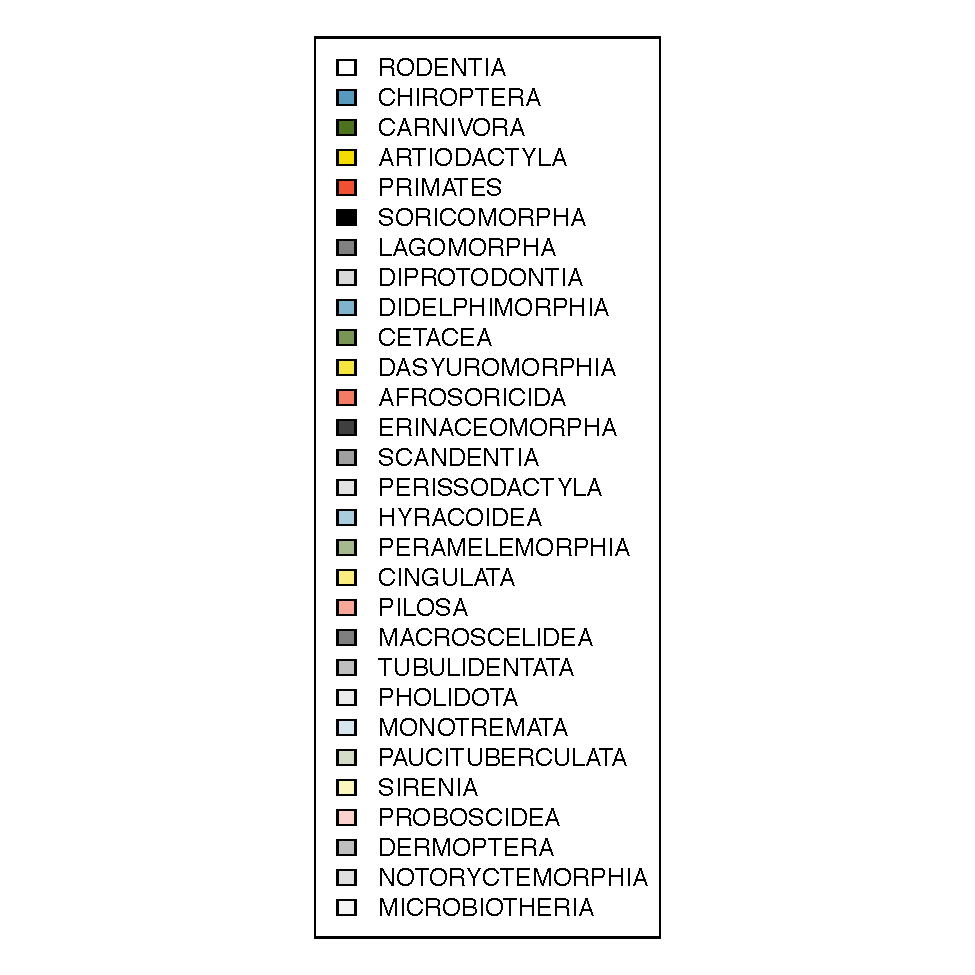
\includegraphics[width=0.2\textwidth]{2-2_categorical_data/figures/mammal_pie_chart/mammal_pie_chart_legend}
\end{center}

\ct{Data from \webURL{http://www.bucknell.edu/msw3}.}

\end{frame}


%%%%%%%%%%%%%%%%%%%%%%%%%%%%%%%%%%%%

\subsection{Comparing numerical data across groups}

%%%%%%%%%%%%%%%%%%%%%%%%%%%%%%%%%%%%

\begin{frame}
\frametitle{Side-by-side box plots}

\dq{Does there appear to be a relationship between class year and number of clubs students are in?}

\begin{center}
\includegraphics[width=\textwidth]{2-2_categorical_data/figures/year_clubs/year_clubs}
\end{center}

\end{frame}

%%%%%%%%%%%%%%%%%%%%%%%%%%%%%%%%%%%%

